% Cohort construction and chronological partitions.
% Counts match the archived cohort/split records described in docs/REPRODUCIBILITY.md.
% Compile with pdfLaTeX. Connectors use named boundary anchors and clear gaps.
\documentclass[tikz,border=5pt]{standalone}
\usepackage[T1]{fontenc}
\usepackage{times}
\usetikzlibrary{arrows.meta,calc}
\definecolor{ink}{HTML}{243B4B}
\definecolor{mainline}{HTML}{688293}
\definecolor{mainfill}{HTML}{F0F5F9}
\definecolor{excludeLine}{HTML}{A68B70}
\definecolor{excludeFill}{HTML}{FAF5EF}
\definecolor{finalLine}{HTML}{4B7C7B}
\definecolor{finalFill}{HTML}{EAF4F2}
\begin{document}
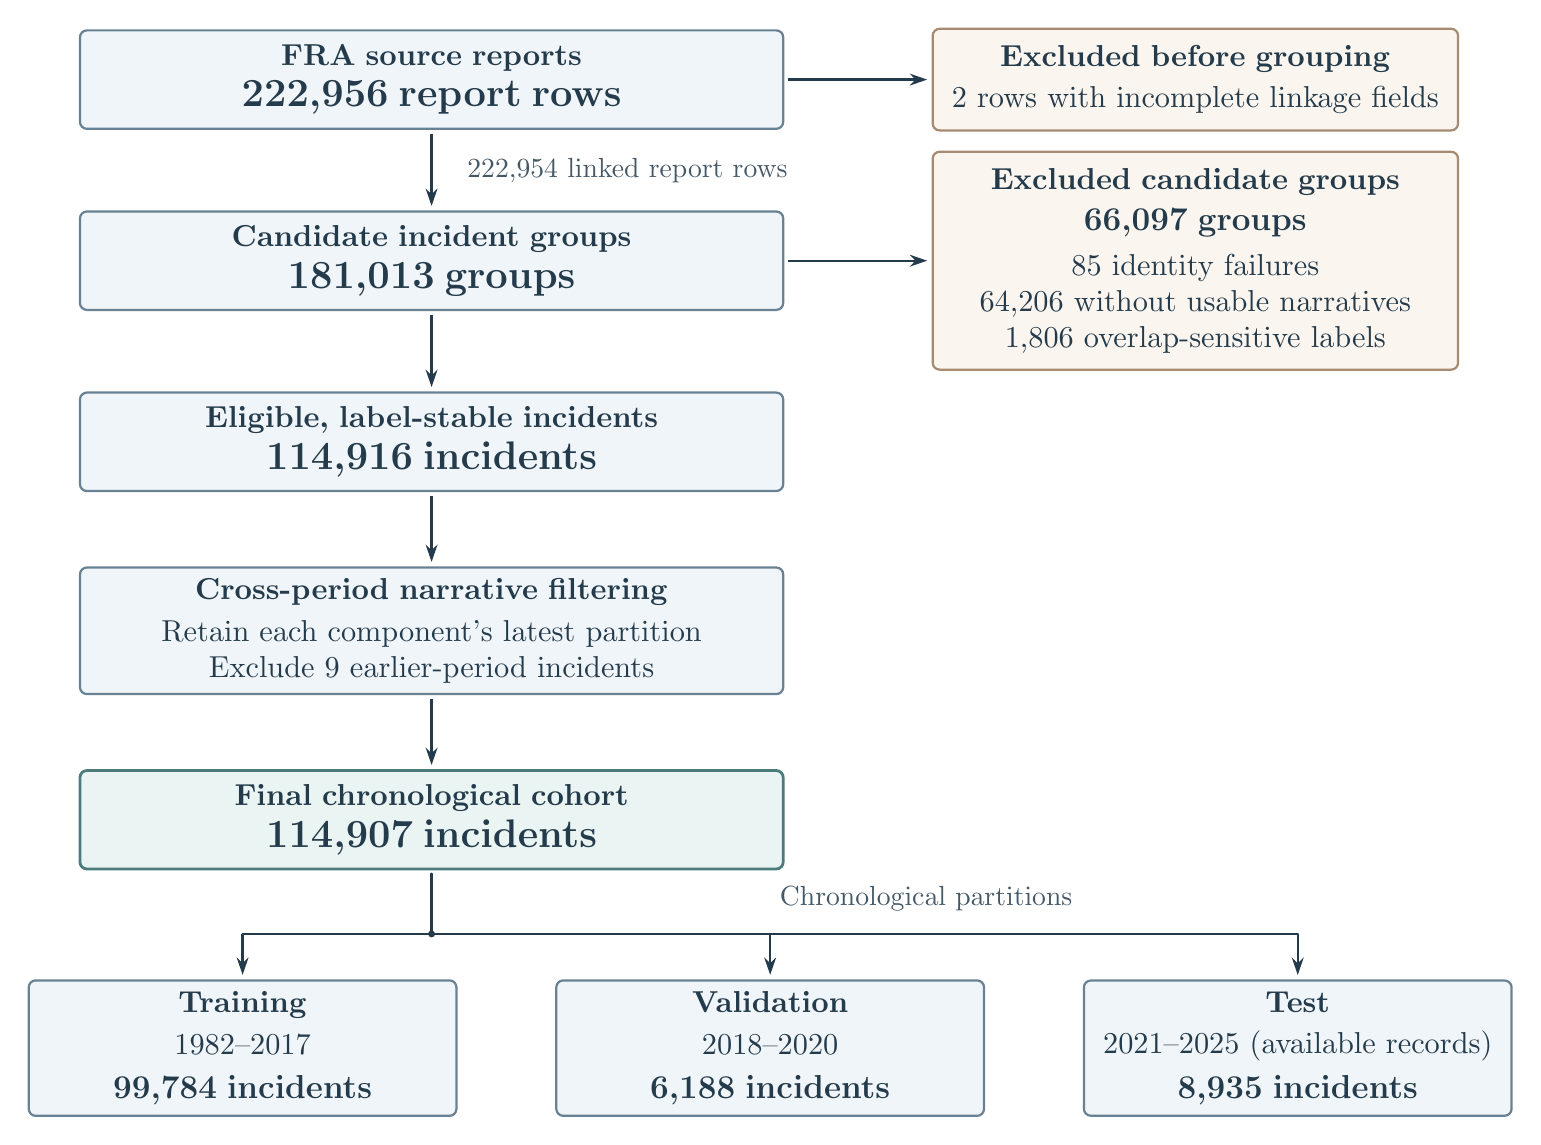
\begin{tikzpicture}[x=1cm,y=1cm,
 font=\fontsize{11}{13}\selectfont,text=ink,
 main/.style={draw=mainline,fill=mainfill,line width=.8pt,
   rounded corners=2.5pt,align=center,text width=8.65cm,
   minimum height=1.25cm,inner sep=4pt,outer sep=0pt},
 exclusion/.style={draw=excludeLine,fill=excludeFill,line width=.8pt,
   rounded corners=2.5pt,align=center,text width=6.25cm,
   inner sep=6pt,outer sep=0pt},
 partition/.style={draw=mainline,fill=mainfill,line width=.8pt,
   rounded corners=2.5pt,align=center,text width=5.15cm,
   minimum height=1.55cm,inner sep=4pt,outer sep=0pt},
 flow/.style={-{Stealth[length=2.2mm,width=1.5mm]},
   draw=ink,line width=.85pt,shorten <=1.7pt,shorten >=2pt},
 branch/.style={draw=ink,line width=.85pt,line cap=round}]

\node[main] (source) at (6.2,12.4)
 {\textbf{FRA source reports}\\[2pt]
  {\fontsize{14}{16}\selectfont\textbf{222,956 report rows}}};
\node[exclusion,minimum height=1.25cm] (incomplete) at (15.9,12.4)
 {\textbf{Excluded before grouping}\\[2pt]
  2 rows with incomplete linkage fields};

\node[main] (candidates) at (6.2,10.1)
 {\textbf{Candidate incident groups}\\[2pt]
  {\fontsize{14}{16}\selectfont\textbf{181,013 groups}}};
\node[exclusion,minimum height=2.20cm] (screened) at (15.9,10.1)
 {\textbf{Excluded candidate groups}\\[2pt]
  {\fontsize{13}{15}\selectfont\textbf{66,097 groups}}\\[3pt]
  85 identity failures\\
  64,206 without usable narratives\\
  1,806 overlap-sensitive labels};

\node[main] (eligible) at (6.2,7.8)
 {\textbf{Eligible, label-stable incidents}\\[2pt]
  {\fontsize{14}{16}\selectfont\textbf{114,916 incidents}}};

\node[main,minimum height=1.55cm] (filter) at (6.2,5.4)
 {\textbf{Cross-period narrative filtering}\\[2pt]
  Retain each component's latest partition\\
  Exclude 9 earlier-period incidents};

\node[main,draw=finalLine,fill=finalFill,line width=1pt] (cohort) at (6.2,3.0)
 {\textbf{Final chronological cohort}\\[2pt]
  {\fontsize{14}{16}\selectfont\textbf{114,907 incidents}}};

% Straight connectors terminate outside the box outlines.
\draw[flow] (source.east) -- (incomplete.west);
\draw[flow] (source.south) -- (candidates.north);
\node[anchor=west,font=\fontsize{10}{12}\selectfont,text=ink!85]
 at (6.53,11.25) {222,954 linked report rows};
\draw[flow] (candidates.east) -- (screened.west);
\draw[flow] (candidates.south) -- (eligible.north);
\draw[flow] (eligible.south) -- (filter.north);
\draw[flow] (filter.south) -- (cohort.north);

% Three equally sized chronological partitions on one row.
\node[partition] (train) at (3.8,.1)
 {\textbf{Training}\\[2pt]1982--2017\\[3pt]
  {\fontsize{13}{15}\selectfont\textbf{99,784 incidents}}};
\node[partition] (validation) at (10.5,.1)
 {\textbf{Validation}\\[2pt]2018--2020\\[3pt]
  {\fontsize{13}{15}\selectfont\textbf{6,188 incidents}}};
\node[partition] (test) at (17.2,.1)
 {\textbf{Test}\\[2pt]2021--2025 (available records)\\[3pt]
  {\fontsize{13}{15}\selectfont\textbf{8,935 incidents}}};

% One orthogonal distribution bus; no connector passes through a box.
\coordinate (junction) at (6.2,1.55);
\draw[branch,shorten <=1.7pt] (cohort.south) -- (junction);
\draw[branch] (3.8,1.55) -- (17.2,1.55);
\fill[ink] (junction) circle[radius=1.25pt];
\draw[flow,shorten <=0pt] (3.8,1.55) -- (train.north);
\draw[flow,shorten <=0pt] (10.5,1.55) -- (validation.north);
\draw[flow,shorten <=0pt] (17.2,1.55) -- (test.north);
\node[anchor=west,font=\fontsize{10}{12}\selectfont,text=ink!85]
 at (10.5,2.0) {Chronological partitions};

\end{tikzpicture}
\end{document}
